% !TeX root =../../main.tex

\chapter{\dFOT: Directed Grey-box Fuzzing} \label{ch:dfot}


\section{Introduction}






Security testing is one of the most effective vulnerability detection techniques for modern software.
Among the security testing techniques, fuzzing~\cite{fuzzing1990}, or fuzz testing, is regarded as the most effective and scalable, which~provides various inputs to the program under test (PUT) and monitors for abnormal behaviors~(e.g., stack or buffer overflow, invalid read/write, assertion failures, or memory leaks)~\cite{fuzzSurvey}. 
Since the proposal, fuzzing has gained the popularity in industry and academia, and evolved into different types of fuzzers for different testing scenarios.
Fuzzers can be classified as black-box, white-box or grey-box~\cite{chen2018systematic}, according to their awareness of the internal structure of the PUT.
Recently, grey-box fuzzers have been widely-used and proven to be effective~\cite{Bohme:2016:CGF}.
Specificaly, AFL~\cite{afl} and its derivations ~\cite{Bohme:2016:CGF,Bohme:2017:DGF,junjie:2017sp:skyfire,2017arXiv170907101L,CollAFL,Angora} receive plenty of attentions.



In general, the existing grey-boxing fuzzers (GFs) aim to cover as many program states as possible within a limited time budget.
However, there exist several testing scenarios in which only particular program states are concerned and required to be sufficiently tested. 
For example, if \emph{MJS}~\cite{mjs}(a JavaScript engine for embedded devices) has a vulnerability discovered on MSP432 ARM platform, similar vulnerabilities may occur in the corresponding code for the other platforms.
In such a situation, the fuzzer should be \emph{directed} to reproduce the bug at these locations.
Another case is, when a bug is patched, the programmers need to check whether the patch completely fixes the bug. 
This requires the fuzzer to focus its efforts on those patched code.
In both scenarios, the fuzzer is required to be directed to reach certain user specified locations in the PUT.
For clarity, we name such locations as \emph{target sites}.
Following the definition in~\cite{Bohme:2017:DGF}, we name the fuzzers that can fulfil the directed fuzzing task as \emph{directed fuzzers}.




As the state-of-the-art directed grey-box fuzzer (DGF for short), {\aflgo}~\cite{Bohme:2017:DGF}~casts the reachability of target sites as an \emph{optimization problem} and adopts a meta-heuristic to promote the test seeds with shorter distances.
Here, the distance is calculated according to the average \emph{weight} of basic blocks on the input seed's execution trace to the target basic block(s), where the weight
 is determined by the edges in the call graph and control flow graphs of the program, and the meta-heuristic is simulated annealing~\cite{kirkpatrick1983optimization}.
Based on these, \aflgo solves the \emph{power scheduling problem} for directed fuzzing --- how many new inputs (termed ``energy'' in \aflgo) should be generated from the current test seed.
To summarize, represented by \aflgo, DGF achieves the goal of reaching the target sites by \emph{combing both static analysis and dynamic analysis}.


A pure dynamic execution can only get the feedback based on the traces it has \emph{already} covered without any awareness about the predefined target sites.
Thus, \textbf{\emph{static analysis}} is required to extract the necessary information for guiding the execution towards the target sites for DGFs. The most widely used approach is to calculate the \emph{distance} (or weight) to the target sites for the components (e.g., basic blocks, functions) of the PUT, so that when executed, DGFs can judge the \emph{affinity} between current seed and the target sites from the components in the execution traces. 
The major challenge is that the distance needs to be effectively calculated without compromising certain desired features.
Particularly, it should help to retain the seed diversity~\cite{Audibert09}.
For example, the existing seed distance calculation algorithm used in \aflgo always favors shortest path that leads to the targets (see \S~\ref{subsec:motiv}), which may starve inputs that could be more easily mutated to reach the target site and further trigger crashes.
The author of libFuzzer~\cite{libfuzzer} argues that not taking into account \emph{all possible traces} may fail to expose the bugs hidden deeply in longer paths~\cite{kcc_aflgo}.
This derives the first desired property \textbf{P1}.
Another challenge is that the static analysis should provide precise information with acceptable overheads.
This is because that coarse static analyses will not benefit the dynamic fuzzing much, while heavyweight static analyses themselves may take considerable time before the dynamic fuzzing starts.
This challenge derives the second desired property \textbf{P2}.
Hence, the first problem is \emph{to have a proper static analysis which can collect necessary information for DGF}.

After extracting the information with static analysis, there are several  challenges in \textbf{\emph{dynamic analysis}} --- how to dynamically adjust different strategies for the purpose of reaching the target sites as fast as possible.
The first challenge is how to properly \emph{allocate} energy to the inputs with different distances and how to \emph{prioritize} the inputs closer to the targets.
This derives the third desired property \textbf{P3}.
The second challenge is how to adaptively change the mutation strategies, since GFs may possess various mutation operators at both coarse-grained (e.g., bulk deletion) and fine-grained (e.g., bitwise flip) levels.
 This derives the fourth desired property \textbf{P4}.
Hence, the second problem is \emph{to make proper adjustments for the dynamic strategies used in DGF}.


To emphasize the two aforementioned problems, an ideal DGF is expected to hold the following desired properties (\S\ref{subsec:dp}):
\begin{enumerate}[\textbf{P}1]
\itemsep0em 
\item The DGF should have a \emph{robust} distance-based mechanism that can guide the directed fuzzing by considering all traces to the targets and avoiding the bias to certain traces.
\item The DGF should strike a \emph{balance} between overheads and utilities in static analysis.
\item The DGF should prioritize and schedule the seeds to reach target sites \emph{rapidly}.\item The DGF should adopt an \emph{adaptive} mutation strategy when the seeds cover different program states. \end{enumerate}


In this paper, we propose our solutions to achieve the four desired properties for DGF. 
For \textbf{P1}, we propose to apply the static analysis results to augment the adjacent-function distance (\S\ref{subsec:functionDist}); and the function level distance and basic block level distance should be calculated based on the augmented adjacent-function distance to simulate the affinities between functions (\S\ref{subsec:UtilityComputation}).
Meanwhile, during fuzzing, we calculate \emph{basic block trace distance} and \emph{covered function similarity} of the execution trace to that of the target functions (\S\ref{subsec:powerSche}) by integrating the static analysis results with the runtime execution information.
For \textbf{P2}, we propose to apply the analysis based on call graph (CG) and control flow graph (CFG), i.e., the function level reachability analysis, the points-to analysis for function pointers (indirect calls), and the basic block metrics (\S\ref{subsec:graghCons}). 
For \textbf{P3}, we propose to combine the basic block trace distance and covered function similarity for solving the power scheduling problem (\S\ref{subsec:powerSche}) and the seed priorization problem (\S\ref{subsec:prioritization}). 
For \textbf{P4}, we propose to apply an adaptive mutation strategy according to the reachability analysis and covered function similarity~(\S\ref{subsec:mutationStr}).

By taking these properties into account, we implemented our DGF, {\dFOT}, and conducted a thorough evaluation with various real-world programs. 
The experimental results show that in most cases, {\dFOT} outperforms the state-of-the-art grey-box fuzzers in terms of the time to reach the target sites and the time to expose the crashes.
Particularly, {\dFOT} can expose certain crashes up to 7 times faster than the state-of-the-art \aflgo, reducing the time to exposure from 3.5 hours to 0.5 hours.

In practice, \dFOT has been successfully discovering crashes with the suspicious target sites reported by other vulnerability detection tools and successfully found more than 41 previously unknown crashes in projects Oniguruma~\cite{oniguruma}, MJS\cite{mjs}, etc. All these vulnerabilities have been confirmed and fixed; among them, 15 vulnerabilities have been assigned unique CVE IDs.

The main contributions of this paper are summarized as follows:
\begin{enumerate}[(1)] 
\itemsep0em
\item We analyzed the challenges in directed grey-box fuzzing and summarized the four desired properties for DGFs.
\item We provided a measure of power function that can guide the fuzzer towards the target sites effectively.
\item We proposed a novel approach to boost the convergence speed to the target sites by utilizing power scheduling, adaptive mutation and seed prioritization.
\item We implemented a novel fuzzing framework that organically combines these ideas and thoroughly evaluated our results in both crash reproduction and target site covering.
\end{enumerate} 

\section{Desired Properties of DGF}\label{sec:mx}

In this section, we first show an example to illustrate the difficulties in DGF.
Based on the observations from the example,~we then propose four desired properties for an ideal DGF.
Finally, we review the state-of-the-art DGF, namely \aflgo~\cite{Bohme:2017:DGF}, with respect~to these four desired properties. 


\subsection{Motivating Example}\label{subsec:motiv}



Fig.~\ref{fig:exam_trace} shows two execution traces related to CVE-2017-15939~\cite{cve-2017-15939}, which is a NULL pointer dereference bug caused by~an incomplete fix in CVE-2017-15023~\cite{cve-2017-15023}.
This vulnerability is difficult for~the~existing GFs to discover.
For instance, AFL~\cite{afl} fails to detect this vulnerability within 24 hours in all the 10 different runs we conducted.
This bug is triggered in \texttt{nm} from GNU binutils.
In function \texttt{concat\_filename}, a NULL pointer is assigned and used without checking, which triggers the segmentation fault.
From a patch testing perspective, we would like to target \texttt{concat\_filename} (subsequently, we will denote this as $T$) and guide the fuzzing to reproduce the crashing trace (i.e., $\langle a, b, c, d, T, Z\rangle$ in Fig.~\ref{fig:call_chain}).




\begin{figure}[t]
	\centering
	\small \begin{tabular}{lcc}
		\hline
  \textbf{Functions in a Crashing Trace} &  	\textbf{File \& Line} & \textbf{Symbol} \\\hline
  	 \texttt{main}   &   \texttt{nm.c} :1794     & \textsf{$M$}\\
 	   ... &  ...  &...  \\
 	 \texttt{\_bfd\_dwarf2\_find\_nearest\_line}     &   \texttt{dwarf2.c} :4798   &  \textsf{$a$}\\
 	 \texttt{comp\_unit\_find\_line}    &   \texttt{dwarf2.c} :3686    & \textsf{$b$}\\
 	 \texttt{comp\_unit\_maybe\_decode\_line\_info} &	 \texttt{dwarf2.c} :3651       &  \textsf{$c$}\\
  	 \texttt{decode\_line\_info}   &    \texttt{dwarf2.c} :2265     &  \textsf{$d$} \\
\texttt{concat\_filename}   &   \texttt{dwarf2.c} :1601     &  \textsf{$T$}\\
    ... 	 	  &     ... 	  &  \textsf{$Z$}\\\hline
	  \textbf{Functions in a Normal Trace} &  	\textbf{File \& Line} & \textbf{Symbol} \\\hline
	   \texttt{main}   &   \texttt{nm.c} :1794     &  \textsf{$M$}\\
	      ... &  ...  &...  \\
	   \texttt{\_bfd\_dwarf2\_find\_nearest\_line}     & \texttt{dwarf2.c} :4798      & \textsf{$a$}\\
	  \texttt{scan\_unit\_for\_symbols}    &      \texttt{dwarf2.c} :3211        &  \textsf{$e$}\\
  \texttt{concat\_filename}   &  \texttt{dwarf2.c} :1601      &  \textsf{$T$}\\
	    ... 	 	  &     ...       & \textsf{$Z$}\\\hline
	\end{tabular}
\vspace{-5pt}
	\caption{Two execution traces related to CVE-2017-15939: $M$ is the main function, $T$ is the target function, $Z$ is the exit.}
	\label{fig:exam_trace}
\end{figure}



For simplicity, in Fig.~\ref{fig:call_chain}, we illustrate only three representative traces for the CVE-2017-15939 by omitting 1) the overlapping functions before $a$ and 2) the other traces that do not pass the target function $T$. {The difficulty in discovering this CVE for the general GFs (e.g., AFL) arises from the fact that the target function $T$ is deeply hidden in the crashing trace.} As shown in Fig.~\ref{fig:call_chain}, the call chain of $\langle a, e, T, Z\rangle$ is shorter than $\langle a, b, c, d, T, Z\rangle$.

Since most of the GFs (such as AFL, LibFuzzer, etc.) are supposed to be \emph{coverage oriented}, and do not care specially about the targets, they may not put most of their efforts in generating test seeds that reach function $T$ and testing the function throughly. For DGFs, although there suppose to be some efforts to guide the fuzzing procedure to favor \emph{some} traces leading to $T$ and focus more on these traces, they may frequently miss \emph{all} the traces. For example, if \aflgo detects that two traces can reach the target sites, it will highly likely favors the trace with shorter path: the distance between the seed to the target is determined by the average distance of the components (basic blocks or functions) in the execution trace to the targets, where the components' distance to the target sites are essentially determined by the number of edges between the components to the targets. This mechanism causes \aflgo to give more energy to the trace $\langle a, e, T, Z\rangle$ since it reaches the target $T$ \emph{and} the induced trace distance is smaller than $\langle a, b, c, d, T, Z\rangle$; on the other hand, less attention is put on $\langle a, b, c, d, T, Z\rangle$, which however causes the crash under some circumstances. Worse still, other traces like $\langle a, e, f, Z\rangle$ may be mistakenly assigned with more energy. As a result, \aflgo was also not able to reproduce the crash within 24 hours in any of the 10 runs we conducted.
 
The challenges of the existing DGF roots in the following aspects: 1) the target functions may appear in several places in PUT, and multiple different traces may lead to the target.  2) since the call graph majorly affects the calculation of the trace distance (the dissimilarity with the target sites), it needs to be accurately built;
in particular, the indirect calls among functions should not be ignored. If the above two issues are not well handled, the distance-based guiding mechanism for DGF will get hindered and fail in such cases.








\subsection{Desired Properties of Directed Fuzzing} \label{subsec:dp}





As observed from the above example, an ideal DGF should possess the following desired properties.




\begin{figure}[t]
	\centering
	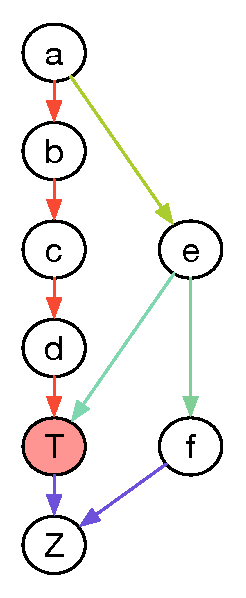
\includegraphics[width=0.2\columnwidth]{res/dfot/eg_callchain.pdf}
	\vspace{-5pt}
	\caption{The fuzzing scenario modeled from Fig.~\ref{fig:exam_trace}: $\langle a, b, c, d, T, Z\rangle $ is a crashing trace passing $T$,  $\langle a, e, T, Z\rangle$ is a normal trace passing $T$, and $\langle a, e, f , Z\rangle$ is a trace not passing $T$.}
	\label{fig:call_chain}
\end{figure}

\subsubsection{\textbf{P1}. The DGF should define a \textbf{robust} distance-based mechanism that can guide the directed fuzzing by avoiding the bias to some traces and considering all traces to the targets.}  \label{subsec:p1}
Different from general GFs, to reach the targets, there may exist several execution traces towards the targets. More often than not, a target function could appear several times in the code and be called even from different entries of the code. Without any static information as guidance, during the fuzzing process, the fuzzer knows nothing about the execution traces that can cover the targets before the targets have been executed; and even if the targets have already been covered, the fuzzer does not know whether there are \emph{other} traces that can lead to these targets.  Hence, the guiding mechanism should help find all the traces that lead to the targets --- taking Fig.~\ref{fig:call_chain} as an example, in the AFL fuzzing process, trace $\langle a, b, c, d, T, Z\rangle$  may not be ever exercised by the existing inputs due to the existence of a strong precondition before $a$. Hence, \emph{the guiding mechanism could provide the knowledge of all possible traces leading to targets and guide the mutation towards it via gradually reducing the distance}. 

However, for DGF, awareness of all possible traces towards the targets is not enough: the distance to the targets for all traces should be properly calculated so that all traces reachable to the targets will be assigned more energy compared to other traces. For Fig.~\ref{fig:call_chain}, $T$ is the target and we would like to check the functionality of $T$\footnote{If we know previously that \emph{only} the traces that involve $d$ and $T$ may cause crashes, we can set \emph{both} $d$ and $T$ as the target sites.}. Intuitively, traces $ \langle a, e, T, Z\rangle$ and $\langle a, b, c, d, T, Z\rangle$ should be treated without bias as both of them can lead to the target site, while $ \langle a, e, f , Z\rangle$ should be less important as it misses the target site. 



\subsubsection{\textbf{P2}. The DGF should strike a \textbf{balance} between overheads and utilities in static analysis.}\label{subsec:p2}  Effective static analysis can benefit the dynamic fuzzing procedure in two aspects: 1) In real world C/C++ programs, there are indirect function calls (e.g., passing a function pointer as a parameter in C, or using function objects and pointers to member functions in C++). In the presence of indirect calls, call sites cannot be observed directly from the source code or binary instructions. So the trade-offs between overheads and utilities need to be made for analyzing them. 2) Not all call relations should be treated equally. For example, some functions occur multiple times in its calling functions, implying  that they have higher chance to be called at runtime. From the static analysis perspective, we need to provide a way to distinguish these scenarios. As to function level distances between functions that have \emph{immediate} calling relations, it is intuitive that callees called in multiple times in different branches should be ``closer'' to the caller.


To sum up, taking Fig.~\ref{fig:call_chain} as an example, \emph{the desired design} for the DGF is: 1) if function $a$ (transitively) calls $T$ in an indirect way (i.e., one or more calls in the chain $a\rightarrow\! b\!\rightarrow\! c\!\rightarrow\! d\!\rightarrow\! T$ are through function pointers), the static analysis should capture such indirect calls, otherwise the distance from $a$ to $T$ will be not available (i.e., treated as unreachable). 2) if the callee appears in more different branches and occurs more times in its caller, a smaller distance should be given since it may have more chance of being called for reaching the target(s). However, modeling the \emph{actual} branch conditions in static phrase is impractical due to the inherent limitations of static analysis. For example, given a nontrivial code segment, it is hard to predict whether the true branch of a predicate will be executed more often than its false branch during runtime. On the other hand, tracking symbolic conditions \emph{dynamically} would be too time costly in a grey-box fuzzing setting.
















\subsubsection{\textbf{P3}. The DGF should select and schedule the seeds to reach target sites \textbf{rapidly}.} \label{subsec:p3}
 AFL determines how many new inputs should be generated (i.e., ``energy'') from a test seed to improve the fuzzing effectiveness (i.e., increase the coverage); this is termed ``power scheduling'' in~\cite{Bohme:2016:CGF,Bohme:2017:DGF}. In directed fuzzing, the goal of fuzzing is not to reach \emph{the upper-limit of coverage} as fast as possible, but reach the \emph{particular targets} as fast as possible. Hence, power scheduling in DGF should determine how many new inputs should be generated from a test seed in order to get a new mutated input that leads to the target sites~\cite{Bohme:2017:DGF}. Similarly, the seed prioritization in DGF is to determine an optimized fuzzing order of test seeds to reach target sites as fast as possible. Both of them can be guided by the distance-based mechanism which measures the affinity between the current seed to the target sites. 
 
 For \emph{power scheduling}, the desired design is that the seed trace with a smaller distance to targets should be assigned more energy for fuzzing, as the trace closer to the target sites gets better chance to reach there. Therefore, $\langle a, e, T, Z\rangle$ should be allocated with similar energy with $\langle a, b, c, d, T, Z\rangle$, and $\langle a, e, f, Z\rangle$ should have less energy than the previous two. For \emph{seed prioritization}, seeds that have smaller distance (``closer'') to the targets should be fuzzed earlier in subsequent mutations. Therefore, $\langle a, e, T, Z\rangle$ and $\langle a, b, c, d, T, Z\rangle$ should be put ahead of $\langle a, e, f, Z\rangle$.

\subsubsection{\textbf{P4}. The DGF should adopt an \textbf{adaptive} mutation strategy when the seeds cover the different program states.}  \label{subsec:p4}
 GFs usually apply different mutations, such as bitwise flip, byte rewrite, chunk replacement, to generate new test seeds from the existing one. 
In general, these mutators can be categorized into two levels: fine-grained mutations (e.g., bitwise flip) and coarse-grained mutations (e.g., chunk replacement).
 Although there is no direct evidence that fine-grained mutations will likely preserve the execution traces, it is widely accepted that a coarse-grained random mutation has a high chance to change the execution trace greatly. Therefore, the desired design is that when a seed has already reached the target sites (including target lines, basic blocks or functions), it should be given less chances for coarse-grained mutations.
 
For the example in Fig.~\ref{fig:call_chain}, consider the case where the DGF has already reached the target function via trace $\langle a, b, c, d, T, Z\rangle $, but crash is not triggered yet.
Now, the DGF should allocate less chances for coarse-grained mutations for the input of $\langle a, b, c, d, T, Z\rangle $.
Meanwhile, if DGF has just started up and $\langle a, b, c, d, T, Z\rangle $ has not been reached yet, then the DGF should give more chances for coarse-grained mutations.
%
 







\subsection{AFLGo's Solution} \label{subsec:aflgo_sol}


In this section, we evaluate the solution of \aflgo against the four desired properties to demonstrate the significances of these properties as well as some useful concepts in DGF.





\begin{figure*}[ht]
	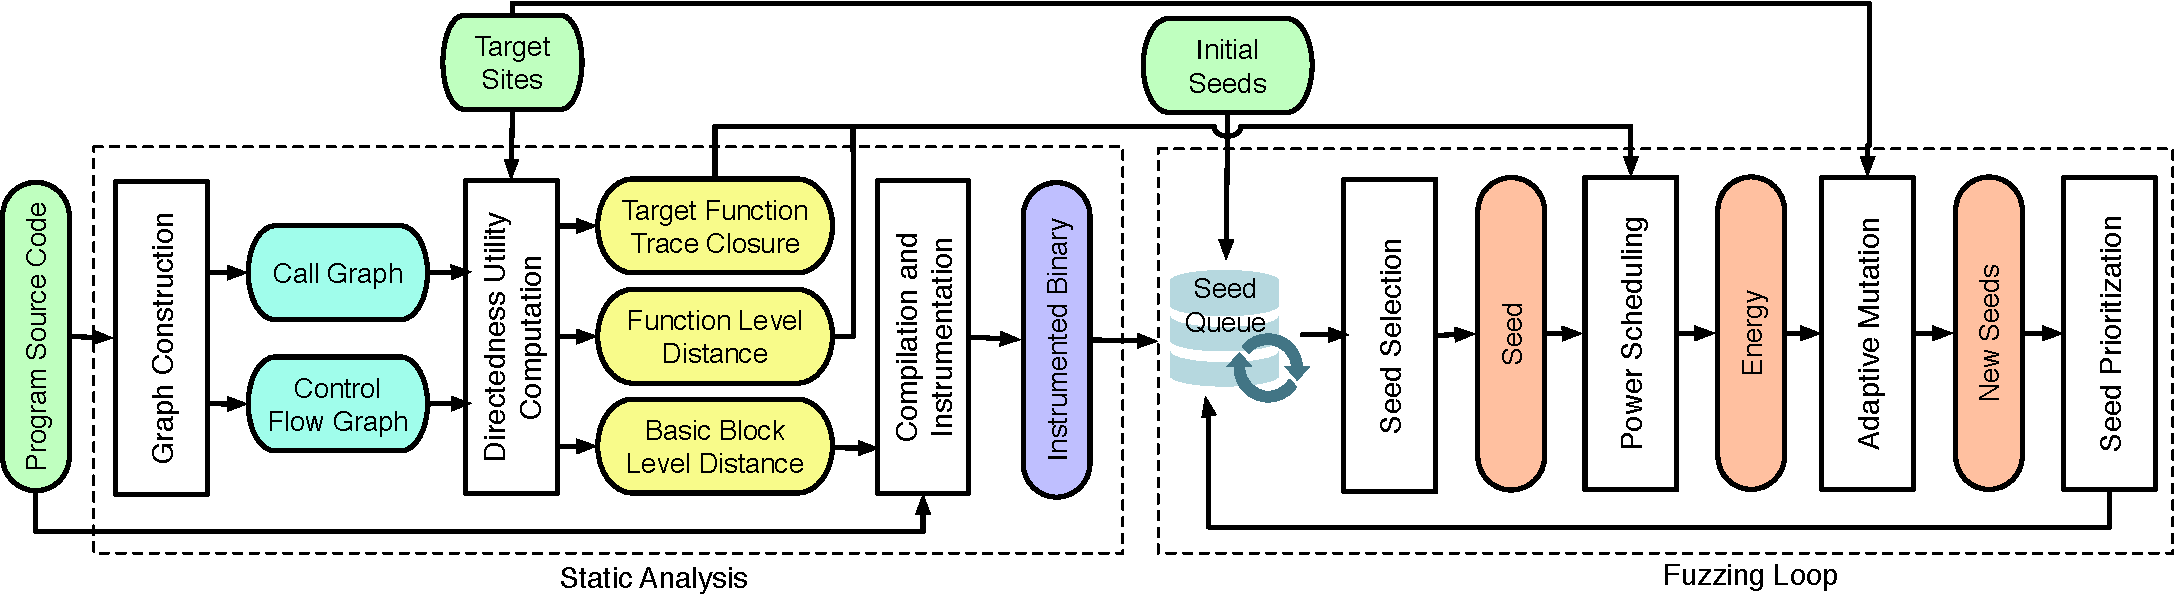
\includegraphics[width=.98\columnwidth]{res/dfot/overview.pdf}
%	\vspace{-20pt}
	\caption{Approach Overview of \dFOT}
	\label{fig:overview}
\end{figure*}

\textbf{For P1.} 
For Fig.~\ref{fig:call_chain}, based on the distance formula defined in \aflgo
the trace distances are:  $d_s(abcdTZ)=(2+3+2+1+0)/5=1.6$, $d_s(aeTZ)=(2+1+0)/3=1$ and $d_s(aefZ)=(2+1)/2=1.5$~\footnote{In fact, \aflgo calculates the trace distance at the \emph{basic block} level with harmonic mean of the accumulative distance; nevertheless, the essential idea is the same.}. 
Given these three execution traces, the energy assigned to them will be $ \langle a, e, T, Z\rangle$ $>$ $\langle a, e, f , Z\rangle$ $>$ $\langle a, b, c, d, T, Z\rangle$.
This is problematic: the normal trace $\langle a, e, T, Z\rangle $ is overemphasized; the crashing trace $\langle a, b, c, d, T, Z\rangle$ is however considered the least important, even less important than the trace $\langle a, e, f , Z\rangle$ that fails to reach the target $T$.



\textbf{For P2.} AFLGo only considers the explicit call graph information.
As a result, all function pointers are treated as \emph{external nodes} which 
are ignored during distance calculation. 
This means that, in an extreme case, if the target function is called via a function pointer, its distance from the actual caller is undefined. 
For example, in Fig.~\ref{fig:call_chain}, if $d$ and $e$ call $T$ via function pointers, both $d$ and $e$ will be mistakenly considered unreachable to $T$; consequently, all nodes except for $T$ will be considered unreachable to $T$. Therefore essentially there is no directedness in such a case.


Besides, \aflgo counts the same callee in its callers only once, and it does not differentiate multiple call patterns between the caller and callee (see \S\ref{subsec:functionDist}).
The function level distance is calculated on the call graph with the Dijkstra shortest path, assuming the weight of two adjacent nodes (functions) in the call graph always to be 1, which will distort the distance calculation. 


\textbf{For P3. } 
\aflgo applies a simulated annealing based power scheduler: it favors those seeds that are closer~to~the targets by assigning more energy to them for mutation; the applied cooling schedule initially assigns smaller weight on the effect of ``distance guidance'', until it reaches the ``exploitation'' phrase. It solves the ``exploration vs exploitation'' problem~\cite{eve} and mitigates the imprecision issue brought by the statically calculated basic block level distance. In our opinion, this is an effective strategy. The problem is that there is no prioritization procedure so the newly generated seeds with smaller distance may wait for a long to be mutated.


 
\textbf{For P4. } The mutation operators of \aflgo come from AFL's two non-deterministic strategies: 1) \emph{havoc}, which does purely randomly mutations such as bit flips, chunk replacement, etc; 2) \emph{splice}, which generates seeds from some random byte parts of two existing seeds. 
Notably, during runtime \aflgo excludes all the deterministic mutation procedures and relies purely on the power scheduling on havoc/splice strategies.
The randomness of these two strategies can indeed favor those with smaller distances to the targets.
However, it may also destroy the existing seeds that are close to the targets.
In fact, some subtle vulnerabilities can only be reached with some special preconditions. In reality, an incomplete fix may still leave some concern cases to be vulnerable; for example, CVE-2017-15939 is caused by an incomplete fix for CVE-2017-15023.
Hence, \aflgo lacks the adaptive mutation strategies, which will mutate arbitrarily even when the current seeds are close to the targets enough.


\textbf{Summary.} Taking \aflgo as example, we can summarize the following suggestions to improve DGFs:

\begin{enumerate}[(1)] 
	\itemsep0em
	\item For \textbf{P1}, a more accurate distance definition is needed to retain trace diversity, avoiding the focus on short traces.
	\item For \textbf{P2}, both direct and indirect calls need to be analyzed; various call patterns need to be distinguished during static distance calculation.
	\item For \textbf{P3}, a moderation to the current power scheduling is required. The distance-guided seed prioritization is also needed. 
	\item For \textbf{P4}, the DGF needs an adaptive mutation strategy, which optimally applies the fine-grained and coarse-grained mutations when the distance between the seed to the targets is different.
\end{enumerate}








 

\section{Approach Overview}

In this section, we briefly introduce the workflow of our proposed approach, named \dFOT. An overview of \dFOT is given in Fig.~\ref{fig:overview}, which~consists of two major components, i.e., \textit{static analysis} and \textit{fuzzing loop}. 



\subsection{Static Analysis}\label{subsec:static_flow}

The inputs of static analysis are the \textit{program source code} and the~\textit{target sites} (i.e., the lines of code that the fuzzer is directed to reach). We derive the basic blocks and functions where the ~target~sites~reside in, and call them \textit{target basic blocks} and \textit{target functions}, respectively. The main output of static analysis is the \textit{instrumented program~binary} with the information of \textit{basic block level distance}.

First, we precisely construct the call graph (CG) of the target~program based on the inclusion-based pointer analysis~\cite{Andersen94programanalysis} to include all possible  calls. Besides, for each function, we construct the  control flow graph (CFG) (\S\ref{subsec:graghCons}).


Second, we compute several~utilities that are used to facilitate the directedness in \dFOT based on CG and CFG (\S\ref{subsec:UtilityComputation}).
\begin{enumerate}[(1)]
\item \textbf{Function level distance} is computed based on CG by augmenting adjacent-function distance (\S\ref{subsec:functionDist}).~This distance is utilized~to calculate the \textit{basic block level distance}. It is also~used during the fuzzing loop to calculate the \emph{covered function similarity} (\S\ref{subsec:powerSche}).
    
\item \textbf{Basic block level distance} is computed based on the function level distance, together with the CG and the functions' CFGs. This distance is statically instrumented for each basic block that is considered to be able to reach one of the target sites. During the fuzzing loop, it is also used to calculate the \emph{basic block trace distance} (\S\ref{subsec:powerSche}).

\item \textbf{Target function trace closure} is computed for each target site~according to the CG to obtain the functions that can reach the target sites. It is used during the fuzzing loop to calculate the \emph{covered function similarity} (\S\ref{subsec:powerSche}).
\end{enumerate}

Finally, the target program is instrumented to keep track of the edge transitions (similar to AFL), the accumulated basic block trace distance (similar to AFLGo), and the covered functions.


\subsection{Fuzzing Loop}\label{sec:fuzz_flow}

The inputs of fuzzing loop are the \textit{instrumented program binary},~the \textit{initial test seeds}, the \textit{target sites} as well as the information of \textit{function level distance} and \textit{target function trace closure}.
The outputs~of~fuzzing loop are the test seeds that cause abnormal program behaviors such as crashes or timeouts.

During fuzzing, the fuzzer selects a seed from a priority seed queue. The fuzzer applies a \textit{power scheduling} against the seed with~the goal of giving those seeds that are considered to be ``closer'' to the target sites more mutation chances, i.e., energy (\S\ref{subsec:powerSche}). Specifically, this is achieved through a power function, which is a combination of the \textit{covered function similarity} and the \textit{basic block trace distance}. For each newly generated test seed during mutation, after capturing its execution trace, the fuzzer will calculate the covered function similarity and the basic block trace distance based on the utilities (\S\ref{subsec:static_flow}). For each input execution trace, its basic block trace distance is calculated as the accumulated basic block level distances divided by the total number of executed basic blocks; and its covered function similarity is calculated based on the overlapping of current executed functions and the target function trace closure, as well as the function level distance.

After the energy is determined, the fuzzer adaptively allocates mutation budgets on two different categories of mutations according to mutators' granularities on the seed (\S\ref{subsec:mutationStr}).
Afterwards, the fuzzer evaluates the newly generated seeds to prioritize those that have more energy or that have reached the target functions (\S\ref{subsec:prioritization}).

%
 

\section{Methodology}

In this section, we will elaborate the key components in Fig.~\ref{fig:overview} featuring the four desired properties.


\subsection{Graph Construction} \label{subsec:graghCons}

To calculate the accurate distance from a test seed to the oracle seed executing the target sites, we first build up the CG and CFG, then combine them to construct the final inter-procedural CFG. Note that CG is used to compute the function level distance in \S\ref{subsec:functionDist} and \S\ref{subsec:UtilityComputation}, CFG together with CG (i.e., inter-procedural CFG) is used to compute the basic block distance in \S\ref{subsec:UtilityComputation}.  	









To identify the indirect call in call graph, we propose to apply the inclusion-based pointer analysis~\cite{Andersen94programanalysis} against the function pointers of the whole program. The core idea of this algorithm is to translate the input program with statements of the form \emph{p := q} to constraints of the form ``\emph{q}'s points-to set is a subset of \emph{p}'s points-to set''. 
Essentially, the propagation of the points-to set is applied with four rules namely \emph{address-of}, \emph{copy}, \emph{assign}, \emph{dereference}. This analysis is context-insensitive and flow-insensitive, meaning that it ignores both the calling context of the analyzed functions and the statement ordering inside functions, and eventually only computes a single points-to solution that holds for all the program points. Usually, a fixed point of the points-to sets will be reached at the end of the analysis. Among these, points-to sets of the function pointers inside the whole program are calculated, resulting in a relatively precise call graph including all the possible direct and indirect calls. The complexity of this pointer analysis is $\Theta(n^3)$.
The reason that we do not apply context-sensitive or flow-sensitive analyses lies in the fact that they are computationally costly and not scalable to large projects. Despite that, our call graph is still much more precise than the one generated by LLVM's builtin APIs, which does not contain any explicit nodes that represent indirect calls. 

The control flow graph of each function is generated based on LLVM's IR. The inter-procedure flow graph is constructed by collecting the call sites in all the CFGs and the CG of the whole program.  By applying these static analyses, we achieve \textbf{P2}.




\subsection{Adjacent-Function Distance Augmentation} \label{subsec:functionDist}
To achieve \textbf{P1}, we propose to implement a lightweight static analysis that considers the patterns of the (immediate) call relation based on the generated call graph.
As discussed in \S\ref{subsec:p2}, under different context, the distances from the calling function to the immediately called function may not be exactly the same. 
Given functions $f_a$, $f_b$, $f_c$, there may exist several different call patterns in the call graph. 
For example, in Fig.~\ref{subfig:dist1} and Fig.~\ref{subfig:dist2}, there are calls $f_a\rightarrow f_b$  and  $f_a\rightarrow f_c$ in both cases. 
However, in Fig.~\ref{subfig:dist1}  $f_a$ is bound to call $f_b$ (since $f_b$ appears in both \emph{if} and \emph{else} branches in $f_a$), but not necessary to call $f_c$; in Fig.~\ref{subfig:dist2}, both $f_b$ and $f_c$ are not necessary to be called by $f_a$.
From a probability perspective, we would think that in both cases the distance from $f_a$ to $f_b$ should be smaller than the distance from $f_a$ to $f_c$, and the distance from $f_a$ to $f_b$ in Fig.~\ref{subfig:dist1} should be smaller than that in  Fig.~\ref{subfig:dist2}. 


\begin{figure}[t]
    \centering
\begin{subfigure}[b]{0.4\columnwidth}
\begin{lstlisting}[language=c]
void fa(int i) {
  if (i > 0) {
    fb(i);
  } else {
    fb(i*2);
    fc();
  }
}
\end{lstlisting}  
\caption{}
\label{subfig:dist1}      
\end{subfigure}
\hspace{0.1in}
\centering
\begin{subfigure}[b]{0.4\columnwidth}
\begin{lstlisting}[language=c]        
void fa(int i) {
  if (i > 0) {
    fb(i);
    fb(i*2);
  } else {
    fc();
  }
}        
\end{lstlisting}
\caption{}
\label{subfig:dist2}      
\end{subfigure}
\caption{An example illustrating different call patterns}
\label{figure:dists}
\end{figure}

Therefore, we propose two metrics to augment the distance that is defined by immediate calling relation between caller and callee.
\begin{enumerate}[(1)] 
\item Call site occurrences \csnum~of a certain callee for a given caller. More occurrences of callee could incur more chance that callee will be dynamically executed with more different (actual) parameters, and in return the distance between the caller to the callee will be smaller. We apply a factor $\Phi(\csnum)=\frac{\phi\cdot \csnum+1}{\phi\cdot \csnum}$ to denote this effect, where $\phi$ is a constant value (usually, $\phi=2$).
\item The number of basic blocks \csbb~in the caller that contains at least one call site of the callee. The rationale is that, with more branches that have a call site, more different execution traces will include the callee. The factor function $\Psi(\csbb)=\frac{\psi\cdot \csbb+1}{\psi\cdot \csbb}$ denotes this effect, and $\psi$ is a constant value (usually, $\psi=2$).
\end{enumerate}

Note that both factor functions are monotone decreasing functions; also, $\Phi$ converges to 1 when $C_N\rightarrow\infty$ and $\Psi$ converges to 1 when $C_B\rightarrow 1$.
Given a (direct or indirect) immediate function call pair $( f_1, f_2)$ where $f_1$ is the caller and $f_2$ is the callee, the original distance between $f_1$ and $f_2$ is 1 (see \aflgo~\cite{Bohme:2017:DGF}). Now, with the two metrics mentioned above, we can define the augmented distance between the function pairs that holds an immediate call relation. The final adjustment factor will be a multiplication of $\Phi$ and $\Psi$, and the \emph{augmented adjacent-function distance} is
\begin{equation}
 \traceFnDistPrime{f_1}{f_2} =  \Psi(f_1, f_2)\cdot\Phi(f_1, f_2)
\end{equation}
where $\traceFnDistPrime{f_1}{f_2}$ refers to the \emph{augmented} \emph{direct} function distance. 

As an example, in Fig.~\ref{subfig:dist1}, for $f_b$, $\csnumn{f_a}{f_b}=2$, $\csbbn{f_a}{f_b}=2$; and for $f_c$, $\csnumn{f_a}{f_c}=1$, $\csbbn{f_a}{f_c}=1$. Assume $\phi=2$ and $\psi=2$ and assume the original distance $\traceFnDist{f_a}{f_b}=\traceFnDist{f_a}{f_c}=1$, the augmented distances will be $\traceFnDistPrime{f_a}{f_c}=\frac{3}{2}\cdot\frac{3}{2}=2.25$, and $\traceFnDistPrime{f_a}{f_b}=\frac{5}{4}\cdot\frac{5}{4}=1.56$.


A special case not shown in the above examples is that some branches form cycles (i.e., loops). Indeed, these functions may be called multiple times at runtime. However, it is uncertain that \emph{how many times} they will be executed across different runs when fed with different seeds. Fortunately, actual execution on one call site of a callee inside one loop typically has similar effect --- the loop explores the similar program states and benefits less in covering new paths. Hence, the function call inside the loop does not bring many execution trace diversities like the scenario where the same callee occurs in multiples branches with significantly different parameters.

The applied approach aims to make a trade-off between the efficiency and the utility of the static analysis. Therefore, we do not consider the solution space of any branch condition that may affect the \emph{runtime reachability} in the CFG. For example, in Fig.~\ref{subfig:dist1}, if we change the condition check \emph{i>0} to be \emph{i==0}, the true branch will be executed only when the input value of $i$ is 0. It is tempting to assign a smaller distance to the code segments in the false branch. However, since the PUT is usually nontrivial, it is impractical to statically formulate the exact constraint set of the preconditions before reaching function $f_a$ and predicate the branches's actual execution probabilities. One common scenario is that the branch condition \emph{i==0} is used for checking the return status code of an external function call, at runtime it may actually execute the true branch more often than the false branch.




\subsection{Directedness Utility Computation} \label{subsec:UtilityComputation}

In \S\ref{subsec:functionDist}, the augmented function distance is calculated on two adjacent functions according to their call patterns. By assigning  the adjacent-function distance as the weight of the edges in the call graph, we can calculate the function level distance for any two functions with the Dijkstra shortest path algorithm, beyond which we can further derive the 
basic block level distance. 
Besides, we also compute the target function trace closure which will be used to calculate the covered function similarity in \S\ref{subsec:powerSche}.

\textbf{Function Level Distance.} This distance is calculated according to CG. It tells the (average) distance from the current function to target functions. Given a function $n$, its distance to the target function set \tgtfnset~is defined as:
\begin{equation}
d_f(n, \tgtfnset) =
\begin{cases}
\textbf{undefined.} & \text{if}~R(n, \tgtfnset)=\emptyset \\
[\Sigma_{\tgtfn\in R(n, \tgtfnset)} \traceFnDist{n}{\tgtfn}^{-1}]^{-1} & otherwise \\
\end{cases}
\label{eq:aflgo_func_dist}
\end{equation}

where $R(n, \tgtfnset) = \left\{\tgtfn | \textbf{reachable}(n, \tgtfn)\right\}$,
which is the set of target functions that can be statically reached from $n$ in CG, and \traceFnDist{n}{\tgtfn} is the \emph{dijkstra shortest path based on augmented function distance} from $n$ to a given target function {\tgtfn} in CG.

\textbf{Basic Block Level Distance.} Given a function $n$ and two basic blocks $m_1$ and $m_2$ inside, the basic block level distance \simpleBBDist{m_1}{m_2} is defined as the minimal number of edges from $m_1$ to $m_2$ in the CFG \cfg{n}.
The set of functions called inside basic block $m$ is denoted as \BBCallees{m},
then $\BBCalleesT{m}=\left\{n | R(n, \tgtfnset)\neq\emptyset, n\in\BBCallees{m} \right\}$, 
and $\transitiveBB=\left\{m| \exists \cfg{n}, m\in \cfg{n}, n\in\fnset, \BBCalleesT{m}\neq\emptyset \right\}$, where $\fnset$ is the set of all functions.
Given a basic block $m$, its distance to the target basic blocks \tgtbbset~are defined as:
\begin{equation}
\traceBBDist{m}{\tgtbbset} = 
\begin{cases}
0 & \textbf{if}~m\in \tgtbbset \\
c\cdot \text{min}_{n\in \BBCalleesT{m}}(\traceFnDist{n}{\tgtfnset})& \textbf{if}~m\in \transitiveBB\\
\Large[\Sigma_{t\in\transitiveBB}\large(\simpleBBDist{m}{t} + \traceBBDist{t}{\tgtbbset}\large)^{-1}\Large]^{-1} & otherwise
\end{cases}
\label{eq:aflgo_bb_dist}
\end{equation}
where $c$ is a constant that magnifies function level distance.

Note that Equation \ref{eq:aflgo_func_dist} and \ref{eq:aflgo_bb_dist}, on their own, are the same as those in \aflgo \cite{Bohme:2017:DGF}. However, $\traceFnDist{n}{\tgtfn}$ for these equations in \aflgo is simply the Dijkstra shortest distance on a CG where the weight of edges (i.e., adjacent function distance) is 1.

\textbf{Target Function Trace Closure.} This utility, $\fntrace{\tgtfnset}$,  is calculated by collecting all the predecessors that can statically lead to the target functions $\tgtfnset$, until the entry function \emph{main} has been reached. We choose \emph{not} to exclude those that are \emph{considered} unreachable from entry function due to the limitations of static analysis. In the example in Fig.~\ref{fig:call_chain}, $\xi_f(T_f)=\{a,b,c,d,e,T\}$.




\subsection{Power Scheduling}  \label{subsec:powerSche}

During dynamic fuzzing, we apply power scheduling on a selected seed based on two dynamically-computed metrics: basic block trace distance and target function trace similarity.

\textbf{Basic Block Trace Distance.} The distance between the seed $s$ to the target basic blocks $\tgtbbset$ is defined as:
\begin{equation}
\traceDist{s}{\tgtbbset} = \frac{\Sigma_{m\in\xi_b(s)}\traceBBDist{m}{\tgtbbset}}{|\bbtrace{s}|}
\label{eq:aflgo_seed_dist}
\end{equation}
where \bbtrace{s} is the execution trace of a seed $s$ and contains all the basic blocks that are executed. Hence, the basic idea of Equation  \ref{eq:aflgo_seed_dist} is that: for all the basic blocks in the  execution trace of $s$, we calculate the average basic block level distance to the target basic blocks  $\tgtbbset$.  Note that Equation \ref{eq:aflgo_seed_dist} is also the same as the one in \aflgo \cite{Bohme:2017:DGF}.

It then applies a feature scaling normalization to get the final distance $\traceDistFinal{s}{\tgtbbset}=\frac{\traceDist{s}{\tgtbbset}-minD}{maxD-minD}$ where $minD$ (or $maxD$) is the smallest (or largest) distances ever met.


\textbf{Covered Function Similarity.} This metric measures the similarity between the execution trace of the seed and the target execution trace \emph{on the function level}. We do not track the basic block level trace similarity since that would introduce considerable overheads. The similarity is calculated based on the intuition that seeds covering more functions in the ``expected traces'' will have more chances to be mutated to reach the targets. This similarity is calculated by tracking the function \emph{sets} the current seed covered (denoted as \fntrace{s}) and comparing it with the target function trace closure $\fntrace{\tgtfnset}$.  In the example in Fig.~\ref{fig:call_chain}, $\xi_f(abcdTZ)=\{a,b,c,d,T\}$, $\xi_f(aeTZ)=\{a,e,T\}$ and $\xi_f(aefZ)=\{a,e\}$.

The covered function similarity is then determined by the following formula:
\begin{equation}
\covDist{s}{\tgtfnset} = \frac{\Sigma_{f\in\fntrace{s}	\cap\fntrace{\tgtfnset}}\traceFnDist{f}{\tgtfnset}^{-1}}{|\fntrace{s}\cup\fntrace{\tgtfnset}|}
\end{equation}

$\traceFnDist{f}{\tgtfnset}$ is the function level distance calculated with Equation~\ref{eq:aflgo_func_dist}. Similar to \traceDistn, a feature scaling normalization is also applied and the final similarity is denoted as \covDistnN. Note that this similarity metric is uniquely proposed in our approach.

\textbf{Scheduling.}
Scheduling deals with the problem how many mutation chances will be assigned to the given seed. The intuition is that if the trace that the current seed executes is ``closer'' to any of the expected traces that can reach the target site in the program, more mutations on that seed should be more beneficial for generating expected seeds. A scheduling purely based on \emph{trace distance} may favor certain patterns of traces. For \aflgo, as mentioned in \S\ref{subsec:p2}, the shorter paths will be assigned more energy, which may starve longer paths that are still reachable to the target sites. To \emph{mitigate} this, we propose the \emph{power function} that considers both \emph{trace distance} (based on basic block level distance) and \emph{trace similarities} (based on covered function similarity): 
\begin{equation}\label{eq:aflgo_power}
p(s, \tgtbbset) = \covDistN{s}{\tgtfnset}\cdot(1 - \traceDistFinal{s}{\tgtbbset})
\end{equation}

It is obvious that the value of $p(s, \tgtbbset)$ fits into $[0,1]$ since both the multipliers are in $[0,1]$.

Compared to AFLGo's approach, which only considers basic block trace distance (\traceDistn, or \traceDistnFinal), our power function balances the effect of shorter paths and the longer paths that can reach the target. Logically, there are some differences between {\covDistn} and {\traceDistn}:
\begin{enumerate}[(1)]
    \item \traceDistn~considers both the effects of CG and the CFGs; {\covDistn} considers only the effects of CG. For \traceDistn, the major effect is still CG due to the magnification factor $c$ used in Equation~\ref{eq:aflgo_func_dist}.
    \item \traceDistn~does not penalize traces that do not lead to the targets, while {\covDistn} penalizes them via a union of \fntrace{s} (by tracking function level traces) and \fntrace{\tgtfnset}.
    \item Given multiple traces that can lead to the targets, {\traceDistn} favors those that have short lengths, but {\covDistn} favors those with longer lengths of common functions in expected trace.
\end{enumerate}

In this sense, $p(s, \tgtbbset)$ strives a balance between shorter traces and longer traces that can reach the target sites with \emph{two heterogeneous metrics}. Admittedly, there may still exist some bias. One of the scenarios is that the power function may assign more energy to a seed that covers many functions in the target function trace closure. For example, assume two traces that can reach the target function $T$: $\langle a,b,c,d,T,Z\rangle$ and $\langle a,e,f,g,T,Z\rangle$; and the target function trace closure is $\langle a, b, c,d,e,f,g,T\rangle$. The power function may assign much energy to a seed with trace $\langle a, b, c, d, e, f, g, Z\rangle$ which does not reach the target function $T$. This is \emph{not} an issue in our opinion: since this seed has covered many ``expected'' functions, it has high chance to be ``close'' to the target; with proper mutations, it is likely to be flipped to mutants that can indeed touch the target.

In {\dFOT}, the power function determines the number of mutation chances to be applied on the current seed (i.e., energy); it is also used during the seed prioritization to determine whether the \emph{mutated} seeds should be favored.


\begin{algorithm}[t]
	\setstretch{0.9}
	\small	
	\SetKwInOut{Input}{input}\SetKwInOut{Output}{output}
	\SetKwInOut{Const}{const.}
	\Input{$s$, the seed to be fuzzed  after power scheduling}
	\Output{$\mathcal{M}_s$, the map to store the new mutated seed, whose key is the seed and whole value is the energy of the seed}
	\Const{$\gamma$, the constant ratio to do fine-grained mutation}
	\Const{$\delta$, the constant ratio to be adjusted}
	\BlankLine
	\SetKw{Continue}{\textbf{continue}}
	\SetKw{And}{\textbf{and}}
	\SetKw{Not}{\textbf{not}}
	\SetKw{Is}{\textbf{is}}
	\SetKw{In}{\textbf{in}}
	\SetKw{Or}{\textbf{or}}
	\SetKw{Eqs}{\textbf{equals}}
	\SetKw{Fori}{\textbf{for}}
	\SetKwProg{Def}{def}{:}{}
$\mathcal{M}_s = \emptyset$\;
	 $p\leftarrow s.getScore()$\; \label{algo1:getscore}
	\If{$ reachTarget(s) == false$}{ \label{algo1:ifcheck}
$\mathcal{S}^{\prime} \leftarrow  coarseMutate(s, p *(1- 	\gamma ))$\; \label{algo1:old_coarse}
	    \For{$s^{\prime}$ in $\mathcal{S}^{\prime}$}{
$\mathcal{M}_s\leftarrow \mathcal{M}_s \cup  \{(s^{\prime},s^{\prime}.getScore())\} $
	    }
   		$\mathcal{S}^{\prime\prime} \leftarrow  fineMutate(s, p * 	\gamma )$\; \label{algo1:old_fine}
    	\For{$s^{\prime\prime}$ in $\mathcal{S}^{\prime\prime}$}{
$\mathcal{M}_s\leftarrow \mathcal{M}_s \cup  \{(s^{\prime\prime},s^{\prime\prime}.getScore())\} $
  		}
	 }
     \Else{ \label{algo1:elsecheck}
     	   
     $\mathcal{S}^{\prime} \leftarrow  coarseMutate(s, p *(1- 	\gamma -\delta ))$\;\label{algo1:new_coarse}
     \For{$s^{\prime}$ in $\mathcal{S}^{\prime}$}{
$\mathcal{M}_s\leftarrow \mathcal{M}_s \cup  \{(s^{\prime},s^{\prime}.getScore())\} $
     }
     $\mathcal{S}^{\prime\prime} \leftarrow  fineMutate(s, p *(	\gamma + \delta))$\; \label{algo1:new_fine}
     \For{$s^{\prime\prime}$ in $\mathcal{S}^{\prime\prime}$}{
$\mathcal{M}_s\leftarrow \mathcal{M}_s \cup  \{(s^{\prime\prime},s^{\prime\prime}.getScore() )\} $
     }
 	}
 
  
	\caption{$adaptiveMutate()$: Adaptive Mutation}
	\label{algo:mutateStr}
\end{algorithm}
 \subsection{Adaptive Mutation} \label{subsec:mutationStr}

In \S\ref{subsec:powerSche}, for each seed, the output of power scheduling is the energy (a.k.a. the times of applied mutations), which will be the input of the step of our adaptive mutation. The problem is that, given the total energy available for a seed, we still need to assign the number of mutations for \emph{each type of mutators}. 


In general, two categories of mutators are used in GFs. Some are coarse-grained in the sense that they change bulks of bytes during the mutations. Others are fine-grained since they only involve a few byte-level modifications, insertions or deletions. For coarse-grained mutations, we consider them to be:
\begin{enumerate}[(1)] 
	\item \textbf{Mixed havoc}. This includes several bulk mutations, namely deleting a chunk of bytes, overwriting the given chunk with other bytes in the buffer, deleting a certain lines, duplicating certain lines multiple times, etc. The actual mutation involves their combinations.
	\item \textbf{Semantic mutation}. This is used when the target program is known to process semantic relevant input files such as javascript, xml, css, etc. In detail, this follows Skyfire~\cite{junjie:2017sp:skyfire}, which includes three meta mutations, inserting another subtree into a random AST position, deleting a given AST, and replacing the given position with another AST.
	\item \textbf{Splice}. This includes a crossover between two seeds in the queue and subsequent mixed havocs.
\end{enumerate}


Algo.~\ref{algo:mutateStr} shows the workflow of our adaptive mutation, given a seed $s$. 
The basic idea is to give less chance of coarse-grained mutations when the seed $s$ can reach the target functions (at line \ref{algo1:elsecheck} in Algo.~\ref{algo:mutateStr}). Once the seed reaches targets, the times of doing fine-grained mutations increase from  $ p * 	\gamma$ (line \ref{algo1:old_fine}) to $p *(	\gamma + \delta)$ (line \ref{algo1:new_fine}), but the times of doing coarse-grained mutation decrease from  $ p *(1- 	\gamma )$ (at line \ref{algo1:old_coarse}) to $p *(1- 	\gamma -\delta )$ (line \ref{algo1:new_coarse}). Here, $s.getScore()$ at line \ref{algo1:getscore} is to get the energy assigned to the seed according to the the power function value calculated in Equation~\ref{eq:aflgo_power}.

\begin{algorithm}[t]
	\setstretch{0.9}
	\small	
	\SetKwInOut{Input}{input}\SetKwInOut{Output}{output}
	\SetKwInOut{Const}{const.}
	\Input{$s$, the seed to be fuzzed  after power scheduling}
	\Input{$i$, the number of iterations to do mutation on the seed}
	\Output{$\mathcal{S}$, the set to store the \emph{new} mutated seed}
	\Const{$\sigma$, the constant ratio to do semantic mutations}
	\Const{$\zeta$, the constant ratio to do mixed havoc mutations}
	\BlankLine
	\SetKw{Continue}{\textbf{continue}}
	\SetKw{And}{\textbf{and}}
	\SetKw{Not}{\textbf{not}}
	\SetKw{Is}{\textbf{is}}
	\SetKw{In}{\textbf{in}}
	\SetKw{Or}{\textbf{or}}
	\SetKw{Eqs}{\textbf{equals}}
	\SetKw{Fori}{\textbf{for}}
	\SetKwProg{Def}{def}{:}{}
	
	$\mathcal{S} = \emptyset$\;	
 	\If{$needSemMutation(s) == true $}{ \label{algo2:checkSem}
 		$\mathcal{S} \leftarrow \mathcal{S} \cup semMutate(s, i * \sigma)$	\;	\label{algo2:applySem}
 		$\mathcal{S} \leftarrow \mathcal{S} \cup coarseHavoc(s, i * (1-\sigma) * \zeta)$\;		\label{algo2:applyHavoc1}
 			$\mathcal{S} \leftarrow \mathcal{S} \cup splice(s, i * (1-\sigma) * (1-\zeta))$	\;	\label{algo2:applysplice1}
}
    \Else{  \label{algo2:checkSemElse}
       	$\mathcal{S} \leftarrow \mathcal{S} \cup coarseHavoc(s, i * \zeta)$\;		\label{algo2:applyHavoc2}
        $\mathcal{S} \leftarrow \mathcal{S} \cup splice(s, i * (1-\zeta))$	\;		\label{algo2:applysplice2}
    }
	\caption{$coarseMutate()$: Coarse-Grained Mutation}
	\label{algo:coarseMutate}
\end{algorithm}
 
$fineMutate()$ in  Algo.~\ref{algo:mutateStr}  simply  applies a random fine-grained mutation (e.g., bit/byte flippings, arithmetics  on some bytes) for the seed. Algo.~\ref{algo:coarseMutate} shows the details for coarse-grained mutation strategy  $coarseMutate()$. Given a seed $s$ and the iteration times of mutations $i$, the basic idea is to apply semantic mutations (line \ref{algo2:checkSem}) only  when it is  necessary (line \ref{algo2:applySem}). The constraints $needSemMutation(s)$ returns true if the following conditions are satisfied: 1) our fuzzer detects that the input file is  a semantic-relevant input file such as javascript, xml, css, etc; 2) The previous semantic mutations have not failed. If not necessary (line \ref{algo2:checkSemElse}), mixed havoc mutations will get more times ($i * \zeta$, at line \ref{algo2:applyHavoc2}) than the necessary case ($i * (1-\sigma) * \zeta$, at line \ref{algo2:applyHavoc1}), and meanwhile splice mutations will also get more times ($ i * (1-\zeta)$ line \ref{algo2:applysplice2}) than necessary ($i * (1-\sigma) * (1-\zeta)$, at line \ref{algo2:applysplice1}).

 In practice, we assign the empirical values to the constants: $\gamma=0.1$, $\delta=0.4$, $\sigma=0.2$, $\zeta=0.8$.



Note that all these new generated  seeds in $\mathcal{M}_s $, together with the original seeds, will be put into the seed queue for future fuzzing. Actually, before fuzzing them, we will prioritize them to improve the efficiency of directed fuzzing (see \S\ref{subsec:prioritization}).




\begin{algorithm}[t]
	\setstretch{0.9}
	\small	
	\SetKwInOut{Input}{input}\SetKwInOut{Output}{output}
	\SetKwInOut{Const}{const.}
	\Input{$s$, the seed to be processed}
	\Output{$\mathcal{Q}_1$, the tier 1 queue to store the most important seeds}
	\Output{$\mathcal{Q}_2$, the tier 2 queue to store the important  seeds}
	\Output{$\mathcal{Q}_3$, the tier 3 queue to store the least important seeds}
	\Const{$\eta$, the threshold of energy value for accepting important seeds}
	\BlankLine
	\SetKw{Continue}{\textbf{continue}}
	\SetKw{And}{\textbf{and}}
	\SetKw{Not}{\textbf{not}}
	\SetKw{Is}{\textbf{is}}
	\SetKw{In}{\textbf{in}}
	\SetKw{Or}{\textbf{or}}
	\SetKw{Eqs}{\textbf{equals}}
	\SetKw{Fori}{\textbf{for}}
	\SetKwProg{Def}{def}{:}{}
	
	$\mathcal{Q}_1 = \mathcal{Q}_2 = \mathcal{Q}_3 = \emptyset$\;	
 	\If{$seedIsNew(s) == true $}{ \label{algo3:checkNew}
  			\If{$seedWithNewEdge(s) == true $}{ \label{algo3:checkNewEdge}
  				$\mathcal{Q}_1 \leftarrow \mathcal{Q}_1 \cup \{s\} $\;	
  			}
  			\ElseIf{$s.powerEnergy() > \eta $}{ \label{algo3:bigEnergy}
  			$\mathcal{Q}_1 \leftarrow \mathcal{Q}_1 \cup \{s\} $\;	
  			}
  			\ElseIf{$reachTarget(s) == true $}{ \label{algo3:reachTarget}
  			$\mathcal{Q}_1 \leftarrow \mathcal{Q}_1 \cup \{s\} $\;	
  			}
  		    \Else{  \label{algo3:checkElse2}
  		    	$\mathcal{Q}_2 \leftarrow \mathcal{Q}_2 \cup \{s\} $\;		 	    	
  		    }
 	}
    \Else{  \label{algo3:checkNewElse}
       	$\mathcal{Q}_3 \leftarrow \mathcal{Q}_3 \cup \{s\} $\;		 
     
    }
	\caption{$seedPrioritize()$: Seed Prioritization}
	\label{algo:seedprioritization}
\end{algorithm}
 


\subsection{Seed Prioritization} \label{subsec:prioritization}

 Not all the seeds have equal or similar priorities, ideally the queue that stores the seeds to be mutated should be a priority queue. However the scoring may be biased (due to the limitations of static analyses, etc.), and the insertion operations on priority queue take a complexity of $\Theta(\log n)$, which is costly since the queue can be quite long and the insertion operation can be frequent. Therefore it is not beneficial \emph{in practice}.\footnote{In fact, the well-known AFL fuzzer only maintains a linked list with some probabilistic to skip seeds that do not cover new edges; the complexity of the  insertion  is $\Theta(1)$.} Instead, we provide a three-tiered queue which appends newly generated seeds into different categories according to their scores. Seeds in the top-tiered queue (tier 1) will be picked firstly, then the second-tiered (tier 2), and finally the lower-tiered (tier 3). This imitates a simplified priority queue with constant time complexity.
 
 
 Algo.~\ref{algo:seedprioritization} shows the seed prioritization strategy for a new seed mutated from the previous step of adaptive mutation. The basic idea is: we should prioritize the \emph{newly generated} seeds that 1) cover new traces 2) have bigger similarity values with the target seeds (i.e., power function values) 3) cover the target functions. We favor the seeds that cover the new traces since we still have to explore \emph{more execution paths} that have the potential to lead to the target sites; this is necessary when the initial seeds are quite far from the targets. The other two prioritization strategies, i.e., comparing similarity values and checking whether the target function have been reached, are specific to directed fuzzing. Note that although these two strategies are relevant, neither of them can be deduced from the other. For the other newly generated seeds, they are put in the second-tiered queue. On the other hand, seeds that have (just) been mutated are assigned with the least priority.
In practice, \dFOT also applies AFL's loop bucket approach (see ~\cite{afl_detail}) to filter out a large number of ``equivalent'' seeds that do not bring new coverage in terms of loop iterations. The prioritization strategies will be applied on the remaining seeds. Therefore, there will not be too many seeds filling up the top-tier queue.

By combining all the static and dynamic techniques mentioned above, for the CVE exampled in \S\ref{subsec:motiv}, \dFOT successfully reproduced the crash with a time budget of 24 hours in 3 out of the 10 runs we conducted when fed with the same initial seeds, which is a significantly improvement on both AFL and AFLGo for this case.
 






%
 

\section{Evaluation}\label{sec:eval}

We implemented our static instrumentation on top of AFL's LLVM mode and the pointer analysis is based on the interprocedural static value-flow analysis tool called SVF~\cite{Sui:2016:SVF}; this part takes about 2000 lines of C/C++ code. The dynamic fuzzer is implemented based on our Rust implementation of AFL. The fundamental framework, called Fuzzing Orchestration Toolkit\cite{fse18-fot}, is written in about 14000 lines of code. We follow exactly AFL's practice~\cite{afl_detail} by using forkserver, shared memory based basic block transition (edge) tracing, deterministic/non-deterministic mutators, etc., and provide a similar user interface as AFL's. The differences, however, are that we design the fuzzer with considerations of modularization and extensibility without sacrifying performance. For directed fuzzing purpose, we add another 4000 lines of code for tracing functions, calculating power function for seeds, distinguishing graininess of mutators, and so on~\footnote{The semantic mutation part is implemented with Antlr~\cite{antlr} in Java ($\sim$4800 lines of code) that is called from Rust via JNI. We didn't enable this mutation strategy in the experiments since this is not tightly relevant to DGF.}. See our website \url{https://sites.google.com/view/ccs2018-fuzz} for more details.

For each program with the given target sites, the instrumentation of {\dFOT} consists of three parts: 1) basic block IDs that track the execution traces 2) basic block distance information that determines basic block trace distance and 3) function IDs that track functions that have been covered. 




\begin{table*}[t]
	\centering
	\caption{Program statistics for our tested programs.}
	\label{tbl:stats}
	\begin{tabular}{c|c|r"r|r|r"r|r"r}
		\thickhline
		\textbf{Project} &  \textbf{Program} &  \textbf{Size} &  \textbf{ics} &  \textbf{cs} &  \textbf{ics/cs} &  \textbf{\# of $C_B$\textgreater1} &  \textbf{\# of $C_N$\textgreater1}  &  \textbf{$t_s$} \\ \hline
		Binutils  &cxxfilt  & 2.8M  & 3232  & 12117 & 26.67\% & 8813  & 8879 &  735s  \\ \hline
		Oniguruma & testcu &	1.3M & 556 & 2065 & 26.93\% & 3037 & 3101 & 5s \\ \hline
		mjs & mjs & 277K & 130 & 3277 & 3.97\% & 309 & 334 & 3s \\ \hline 
		libjpeg & libjpeg & 810K & 749 & 1827 & 41.00\% & 144 & 152 & 2s \\ \hline
		libpng & libpng & 228K &  449 & 1018 & 44.11\% & 61 & 61 & 2s \\ \hline
		freetype2 & freetype & 1.6M & 627 & 5681 & 11.30\% & 6784 & 7117 & 4s \\ \thickhline                         
	\end{tabular}
\end{table*}

\subsection{Evalution Setup}\label{subsec:evalsetup}

In the experiments, we aim to answer the following questions:

\begin{enumerate}[\textbf{RQ}1]
    \item  Is the static analysis really worth the effort?
    \item  How good is {\dFOT}'s performance in terms of reproducing the target crashes?
    \item  How effective are the dynamic strategies in {\dFOT}?
    \item  How good is the ability of {\dFOT} for reaching the specific target sites?  
\end{enumerate}

\textbf{Evaluation Dataset.}
We evaluated \dFOT with diverse real-world programs:
\begin{enumerate}[(1)] 
    \item \textbf{GNU Binutils}~\cite{binutils} is a collection of binary analysis tools used in GNU/Linux platform. 
This benchmark is also used in several other works such as~\cite{Bohme:2016:CGF, Bohme:2017:DGF, 2017arXiv170907101L}.
    \item \textbf{MJS}~\cite{mjs} is an embedded JavaScript engine for C/C++ and used in IoT development.
    It is used to compare \dFOT directly with {\aflgo} due to implementation limitations of the latter.
    \item \textbf{Oniguruma}~\cite{oniguruma} is a versatile regular expression library used by multiple world famous projects such as PHP~\cite{php}.
    \item \textbf{Fuzzer Test Suite}~\cite{fuzzer-test-suite} is a set of benchmarks for fuzzing engines.
    It contains several representative real-world projects.
\end{enumerate}

\textbf{Evalution Tools.} We compare {\dFOT} with the following three fuzzers:
\begin{enumerate}[(1)] 
\item \textbf{AFL} is the current state-of-the-art GF. It ignores all the target information for the PUT and only does the ``basic block transition'' instrumentation.
\item \textbf{{\aflgo}} is the state-of-the-art DGF based on AFL.
Compared to AFL, it also instruments basic block distance information.
\item \textbf{{\dGO}} is the fuzzer where the basic block level distance is generated with our static analysis procedure (Fig.~\ref{fig:overview}), but the dynamic fuzzing is conducted by {\aflgo}.
\end{enumerate}

Here we mainly follow \aflgo's practice to only use AFL as the baseline for coverage oriented GFs. Other techniques do not focus on directed fuzzing, and they are either orthogonal (e.g., CollAFL~\cite{CollAFL}) or may sometimes perform worse than AFL (e.g., \aflfast, as observed by \cite{Shastry:LNCS2017:Orthrus}), or not publicly available (e.g., Angora~\cite{Angora}). The detailed reason is available at our website. %; in \S\ref{sec:related}, we also provide a more detailed comparison between {\dFOT} and these techniques.

In the experiments, all AFL based fuzzers (AFL, {\aflgo} and {\dGO}) are run in their ``fidgety'' mode~\cite{FidgetyAFL}. For both {\aflgo} and {\dGO}, ``time-to-exploitation'' is set to 45 minutes for the fuzzer. Except for the experiments against GNU Binutils (Table~\ref{tbl:cr_aflgo_binutils}) , where we follow exactly the setup in {\aflgo}'s paper~\cite{Bohme:2017:DGF} , all the other experiments are repeated 8 times, with a time budget of 4 hours. 
We use ``time-to-exposure'' (TTE) to measure the length of the
fuzzing campaign until the first test input is generated that triggers a given error (in~\S\ref{subsec:evalcrashrepro}) or reaches a target site (in~\S\ref{subsec:evalsrcloc}).
We use \emph{hitting round} to measure the number of runs in which a fuzzer triggers the error or reaches the target.
For all the experiments, if the fuzzer cannot find the target crash within the time budget in one run, TTE is set to the time budget value. 

Our experiments are conducted on an Intel(R) Xeon(R) CPU E5-2697 v3 @ 2.60GHz with 28 cores, running a 64-bit Ubuntu 16.04 LTS system; during experiments, we use 24 cores and retain 4 cores for other processes. 


\subsection{Static Analysis Statistics}\label{subsec:evalstatic}


In Table~\ref{tbl:stats}, the first three columns denote the projects, programs and the sizes in their LLVM bitcode form. \emph{ics} denotes the number of indirect call sites in the binary, which is calculated by counting those call sites without explicitly known callees; \emph{cs} is the number of call sites; \emph{ics/cs} denotes the percentage of indirect calls among all call sites. 
The next two columns denote the number where $C_B>1$ and $C_N>1$ (\S~\ref{subsec:functionDist}), respectively. The last column denotes the time cost of call graph generation, which takes the majority of the time among all the directedness utility computation.



We can see from  the table that the chosen targets have fair diversities in terms of different metrics.
It is also noticeable that the number of indirect function calls may contribute a large portion to the total number of function calls.
Specifically, in libpng, $44.11\%$ function calls are indirect function calls.
This clearly shows the importance of building precise call graphs.
Furthermore, the number of occurrences of $C_N>1$ and the number of occurrences of $C_B>1$ are also large, which shows the importance of taking into consideration the different patterns of call relations.




As to the overhead of the static directedness utility computation, except for \emph{cxxfilt}, which requires approximately 12.5 minutes to generates the call graph, call graphs of most other projects can be generated in seconds. For cxxfilt, the performance degradation lies in the inherent complexity of the project itself. From the program statistics in Table~\ref{tbl:stats}), it is obvious that the code base is bigger and the program structures are more complicated than the others. In fact, the bottleneck of the analysis is inside the pointer analysis implemented in SVF tool. We believe that it is worth the effort due to the fact that this procedure is done purely statically. And as long as the source code does not change, the call graph can be reused.


%
 
\subsection{Crash Exposure Capability}\label{subsec:evalcrashrepro}

The most common application of directed fuzzing is to try to expose the crash with some given suspicious locations that are supposed to be vulnerable, where the suspicious locations can be detected with the help of other static or dynamic vulnerability detection tools.
In this experiment, we directly compare {\dFOT} with other fuzzers on some known crashes to evaluate its crash exposure capability.

\subsubsection{Crash Reproduction against Binutils}

In the beginning, we intended to compare GNU Binutils directly with {\aflgo} in our experiments since it is an important benchmark in ~\cite{Bohme:2017:DGF} to demonstrate {\aflgo}'s directedness. However, we found that the actual implementation of {\aflgo} has a few issues~\cite{aflgo_issues} in generating static distances. Most importantly, it takes too long to calculate the distances. As a result, when we tried {\aflgo}'s static analysis on GNU Binutils 2.26, it failed to generate ``distance.cfg.txt'' which contains the distance information for instrumentation within 12 hours\footnote{{Besides the performance issue of \aflgo, another reason to reclaim \aflgo's results in Table \ref{tbl:cr_aflgo_binutils} is that the hardware environments are similar. The reason is supported by the similar results produced by AFL in \textbf{~\cite{Bohme:2017:DGF}} and our experiments.}}. Although {\aflgo} can still perform fuzzing without distance information instrumentation, the fuzzing process is no longer \emph{directed} without any distance input.
Therefore, we reclaimed the results in~\cite{Bohme:2017:DGF} to compare with ours for the GNU Binutils benchmark~\footnote{Since CVE-2016-4487/CVE-2016-4488 and CVE-2016-4492/CVE-2016-4493 share the same target sites, we treat them as the same; the reclaimed value for CVE-2016-4487/CVE-2016-4488 are also average values.}. We follow exactly the evaluation setup in~\cite{Bohme:2017:DGF} where each experiment is conducted for 20 times, with the time budget set as 8 hours; the initial input seed file only contains a line break (generated by \verb|echo "" > in/file|). The target sites we specified are based on their CVE descriptions and the backtraces of the crashes. We compare {\dFOT} with {\aflgo} and AFL; the results are shown in Table~\ref{tbl:cr_aflgo_binutils}. In {\aflgo}'s paper, the {\alz} metric~\cite{alz_metric} is used to show the possibility that one fuzzer is better than the other according to all the runs. It is ignored in Table~\ref{tbl:cr_aflgo_binutils} since we cannot get the result of each run in their experiments.

\begin{table}[t]
    \small
\centering
\caption{Crash reproduction in {\dFOT}, {\aflgo} and AFL against Binutils.}
\label{tbl:cr_aflgo_binutils}
     \begin{tabular}{c"c|r|r|c}
         \thickhline
    \textbf{CVE-ID}   & \textbf{Tool}  & \textbf{Runs} & \utte (s)  & \textbf{Factor} \\ \thickhline
    \multirow{3}{*}{\begin{tabular}[c]{@{}l@{}}2016-4487\\ 2016-4488\end{tabular}}& Hawkeye &   20    &   177   & -- \\ \cline{2-5} 
    & AFLGo  &  20  & 390 & 2.20\\ \cline{2-5} 
    &  AFL   &   20 & 630  &   3.56  \\ \hline
    \multirow{3}{*}{2016-4489} & Hawkeye & 20  &  206 & --  \\ \cline{2-5} 
     & AFLGo  &  20 &180&  0.87 \\ \cline{2-5} 
     & AFL   &   20  &  420  &   2.04  \\ \hline
    \multirow{3}{*}{2016-4490}  & Hawkeye & 20 & 103  &  -- \\ \cline{2-5} 
    & AFLGo  &  20 & 93   & 0.90  \\ \cline{2-5} 
    &   AFL   &  20 &  59   &  0.57  \\ \hline
    \multirow{3}{*}{2016-4491} & Hawkeye &  9  & 18733 &   --   \\ \cline{2-5} 
    &   AFLGo  &  5 & 23880    &    1.27     \\ \cline{2-5} 
    &        AFL   &       7    &            20760    &            1.11   \\ \hline
    \multirow{3}{*}{\begin{tabular}[c]{@{}l@{}}2016-4492\\ 2016-4493\end{tabular}} & Hawkeye &     20      &                    477                                 &       --      \\ \cline{2-5} 
    &   AFLGo  &     20   &  540  &                 1.21                                               \\ \cline{2-5} 
    &    AFL   &     20   &                         960                            &                  2.01                                              \\ \hline
    \multirow{3}{*}{2016-6131} & Hawkeye &       9     &                     17314                                &                      --                                          \\ \cline{2-5} 
    &   AFLGo  &                   6                                   &                      21180                               &                                1.22                                \\ \cline{2-5} 
     & AFL   &                    2                                  &            26340                                         &             1.52                                                   \\ \thickhline
    
\end{tabular}  
\end{table}

We can observe the following facts: 
1) For CVE-2016-4491 and CVE-2016-6131, \dFOT achieves the best results, with the most hitting rounds (both are 9 rounds) and the shortest {\utte} (18773s and 17314s). Compared with other tools, on average for both cases, \dFOT's improvements are significant in term of hitting rounds ($>20\%$) and {\utte} ($>20\%$).
2) For CVE-2016-4487/4488 and CVE-2016-4492/4493, all tools reproduce the crashes in 20 runs, and \dFOT achieves the best {\utte}. Specifically, on these two cases, \dFOT's improvement in terms of {\utte} is significant --- reducing at least $20\%$ than other tools.
3) For CVE-2016-4489 and CVE-2016-4490, all tools reproduce the crashes in all runs within 7 minutes since these bugs are relatively easy to find. 
Apparently, in such cases, directed fuzzers have no significant advantage --- in other words, when the crashes are shallow or easy to trigger, \dFOT's merits cannot show and fuzzing randomness matters for \utte.

To summarize, {\dFOT} has the real potential to fulfill directed fuzzing tasks where the target crashes are not easy to be detected.

\subsubsection{Crash Reproduction on MJS}

In order to \emph{directly} compare the performance between {\dFOT} and {\aflgo}, we chose a project called \emph{MJS}, which contains a single source file and the results are in Table~\ref{tbl:cr_aflgo_mjs}.
We used this project for direct comparison with \aflgo since \aflgo took too much time or failed to generate the distance information for other projects such as Oniguruma, libpng, etc. 
On \emph{MJS}, \aflgo took an average of 13 minutes to generate the basic block distance for different targets.
During experiments, the initial input seed files are all from the project's \emph{tests} directory. The targets are selected from the crashes reported in the project's GitHub pages, which correspond to four categories of vulnerabilities, namely \emph{integer overflow} (\#1), \emph{invalid read} (\#2), \emph{heap buffer overflow} (\#3), and \emph{use after free} (\#4). We can observe the following facts : 
1) On \#1 and \#2,  \dFOT achieves the best results, with the most hitting rounds and the shortest {\utte} for both cases.  In terms of hitting rounds, {\dFOT} found \#1's bug in 5 runs and \#2's bug in 7 runs, while for the other two tools they only detected both crashes in 2 runs. Notably, this case is nontrivial and {\dFOT} reduces the {\utte} from about 3.5 hours to 0.5 hours.
2) On \#3, for which all the tools reproduce the crash in 8 rounds. Still, \dFOT has the highly significant improvement on {\utte}, using less than one fourth {\utte} of other tools.
3) On \#4, all the tools reproduce the crash in all rounds, and the {\utte} differences among them are not significant.
As to \alz, we can see that \dFOT exhibits really good results, for  example, the values in \#2 are both 0.95, which means \dFOT has 95\% confidence to perform better than both other tools.



 \begin{table}[t]
    \small
    \centering
    \caption{Crash reproduction in {\dFOT}, {\aflgo} and AFL against MJS.}
    \label{tbl:cr_aflgo_mjs}
    \begin{tabular}{c|c|c|r|c|c}
        \thickhline
        \textbf{Bug ID}                                                                                                                                  & \textbf{Tool}  & \textbf{Runs} & \utte (s) & \textbf{Factor} & \alz \\ \thickhline
        \multirow{3}{*}{\#1} & Hawkeye &       5                                               &         5469                                            &             --                                 & --                  \\ \cline{2-6} 
        &             AFLGo  &         2                                             &                              12581                       &                  2.30                             &     0.77            \\ \cline{2-6} 
        &             AFL   &        2                                              &                              13084                       &                       2.39                        &     0.77            \\ \hline
        \multirow{3}{*}{\#2}  & Hawkeye &       7                                               &                    1880                                 &             --                               & --                    \\ \cline{2-6} 
        &            AFLGo  &             2                                         &                    12753                                 &                6.78                           &          0.95           \\ \cline{2-6} 
        &        AFL   &             2                                         &                   12294                                  &               6.54                           &          0.95            \\ \hline
        \multirow{3}{*}{\#3} & Hawkeye &                           8                           &      178                                               &           --                     & --                                \\ \cline{2-6} 
        &       AFLGo  &         8                                             &                       819                              &                       4.60                      &           0.91        \\ \cline{2-6} 
        &        AFL   &            8                                          &                         1269                            &                     7.13                   &              0.95          \\ \hline
        \multirow{3}{*}{\#4}  & Hawkeye &      8                                                &                 5519                                    &              --                         & --                         \\ \cline{2-6} 
        &       AFLGo  &                8                                      &                 5878                                    &             1.07                                 &    0.57              \\ \cline{2-6} 
        &       AFL   &             8                                         &                 5036                                    &             0.91                              &    0.48                 \\ \thickhline          
    \end{tabular}  
\end{table}

\subsubsection{Crash Reproduction on Oniguruma}

Here we compare \dFOT with \dGO on Oniguruma to show the advantage of dynamic analysis strategies in \dFOT.
Therefore, the major differences between {\dFOT} and {\dGO} is mainly the dynamic part.
Due to the aforementioned performance issues of \aflgo~in static analysis on Oniguruma and other big projects, hereinafter, we will used \dGO as an alternative	to \aflgo in the subsequent experiments.
We therefore compare {\dFOT} with {\dGO} to show the effectiveness of our dynamic strategies.

In Table~\ref{tbl:exp_onig}, we compare \dFOT with \dGO and AFL against the Oniguruma regex library. The first three bugs come from the reported CVEs which occur on version 6.2.0, and Bug \#4 is an newly fixed vulnerability issue on its GitHub pages.
Some observations are: 
1) For \#3 and \#4,  \dFOT achieves the best results among the three tools. 
Especially, for \#4, the improvements in both hitting rounds and  {\utte} are highly significant. 
For \#3, \dFOT can find the bug in one more round, but the {\utte} is similar for the three tools.
2) For \#1 and \#2,  all the tools reproduce the crash in 8 rounds. On the other hand, \dFOT and \dGO have no significant differences in {\utte}.
From the results, we can conclude that the dynamic analysis strategies used in \dFOT are effective.







 

\begin{table}[t]
    \small
    \centering
    \caption{Crash reproduction on {\dFOT}, {\dGO} and AFL against Oniguruma.}
    \label{tbl:exp_onig}
    \begin{tabular}{c|c|c|r|c|c}
        \thickhline
        \textbf{Bug ID}                                                                                                                      & \textbf{Tool}  & \textbf{Runs} & \utte  (s) & \textbf{Factor} & \alz \\ \hline
        \multirow{3}{*}{\#1}  & Hawkeye &                      8                                &            139                                         &                     --                         & --                  \\ \cline{2-6} 
        &               HE-Go  &   8                                                   &                     149                                &           1.07                     &          0.58                       \\ \cline{2-6} 
        &        AFL   &   8                                                   &                            135                         &                          0.97                       &       0.54         \\ \hline
        \multirow{3}{*}{\#2} & Hawkeye &                       8                               &           186                                          &                       --                   & --                      \\ \cline{2-6} 
        &          HE-Go  &       8                                              &                     228                                 &                  1.23                        &         0.88             \\ \cline{2-6} 
        &    AFL   &         8                                             &                        372                             &                 2.00                        &        1.0               \\ \hline
        \multirow{3}{*}{\#3} &  Hawkeye &                               2                       &            13768                                         &                   --                     &        --                \\ \cline{2-6} 
        &     HE-Go  &       1                                               &                              14163                       &                         1.03                 &        0.56              \\ \cline{2-6} 
        &      AFL   &        1                                              &                              14341                       &                    1.04                       &        0.57             \\ \hline
        \multirow{3}{*}{\#4} &  Hawkeye &                  7                                    &                6969                                     &                  --                 & --                             \\ \cline{2-6} 
        &      HE-Go  &       3                                               &                      12547                               &                 1.80                         &          0.82             \\ \cline{2-6} 
        &       AFL   &              1                                       &                  14375                                &             2.06                            &           0.88            \\ \thickhline
        
    \end{tabular}
\end{table} 


\subsection{Target Site Covering}\label{subsec:evalsrcloc}
Certain locations in the PUTs are hard to reach, though they may not trigger crashes.
In practice, the generated seeds that can cover the such locations can also be used as initial seeds for CGFs to boost their coverage. 
Therefore, this criterion is an important factor for measuring DGFs' capabilities. 

Google's fuzzing test suite contains three projects that specially focus on testing fuzzers' abilities of discovering hard to reach locations, namely \emph{libjpeg-turbo-07-2017} (\#1), \emph{libpng 1.2.56} (\#2, \#3) and \emph{freetype2-2017} (\#4). 
In these benchmarks, the target sites are specified by file names with line numbers in the source files. 
Here we manually added some additional ``sentinel'' code in the target sites (``exit(n)'', where the values of `n` distinguish these sites) to indicate that the relevant targets have been reached. 


Table~\ref{tbl:discover_src} shows the results on these benchmarks. 
Case \#1 and \#4 show that \dFOT exhibits good capability in terms of rapidly covering the target sites, according to {\utte}~and the factor columns; considering \alz, the behaviors are also steady. 
In case \#2 and \#3, it takes little time to reach these target sites for all the fuzzers.
While on the relevant project page~\cite{libpng-fts}, it is mentioned clearly that they ``currently require too much time to find''. 
We actually tried this benchmark on libFuzzer with the default scripts in 2 machines, indeed it failed to reach the target sites. 
This root cause of the inconsistency may lie in the fact that the inner mechanisms may affect the actual fuzzing effectiveness (In fact, libFuzzer is known to be quite different from AFL and its derivations). The other observation is that {{\dGO}} has a rather big value in terms of {\utte} compared to other tools. It turns out that in one of the runs, the TTE is 524s, much larger than all the other runs.

It is worth noting that the \utte~to cover the target sites (Table \ref{tbl:discover_src}) is \emph{quite} different from the {\utte} to trigger real-world crashes (Table \ref{tbl:exp_onig}): the TTEs of the former are calculated based on the duration to cover the specific \emph{line} at the first time; while the TTEs of the latter are tightly relevant to \emph{branch coverage} or even \emph{path coverage} since typically bugs in widely used software can only be triggered with special path conditions and it requires covering a few execution traces. Although Table \ref{tbl:discover_src} shows that \dFOT's improvements against \dGO in covering target sites are not obvious (and for a few cases, it performs worse), we can observe in Table \ref{tbl:exp_onig} the acceleration on crash reproduction is significant specially for \#4 (1.80x, nearly 2 hours off) and \#2 (1.23x). This actually indicates that dynamic strategies are quite effective in \emph{detecting crashes}.

\begin{table}[t]
	\small
	\centering
	\caption{Target site covering results in \dFOT, \dGO and AFL against Fuzzer Test Suite  (libjpeg-turbo, libpng, freetype2).}
	\label{tbl:discover_src}
	\begin{tabular}{c|c"c|c|r|c|c}
		\thickhline
		ID                                                              & Project                                                                    & Tool  & Runs & \utte (s) & Factor &  \alz \\ \hline
		\multirow{3}{*}{\#1} &\multirow{3}{*}{jdmarker.c:659}  & {\dFOT} &                     8                                 &           1955                                          &                               --                      & --           \\ \cline{3-7} 
		&                                                                            & HE-Go  &           8                                           &                    2012                                 &             1.03                                                 &  0.53 \\ \cline{3-7} 
		&                                                                            & AFL   &       8                                               &                 4839                                    &              2.48                                               &  0.95   \\ \hline
		\multirow{3}{*}{\#2} & \multirow{3}{*}{pngread.c:738} & {\dFOT} &                            8                          &                            23                         &                               --                  & --               \\ \cline{3-7} 
		&                                                                            & HE-Go  &              8                                        &                         16                            &                 0.70                                           &  0.43   \\ \cline{3-7} 
		&                                                                            & AFL   &               8                                       &                              130                       &                   5.65                                      &    1.00   \\ \hline
		\multirow{3}{*}{\#3} &\multirow{3}{*}{pngrutil.c:3182} & {\dFOT} &    8                                                  &                                   1                  &                               --                         & --        \\ \cline{3-7} 
		&                                                                            & HE-Go  &                     8                                 &                           66                          &                               66.00                        &    0.56      \\ \cline{3-7} 
		&                                                                            & AFL   &                     8                                 &                      3                               &                      3.00                             &     0.51        \\ \hline        
		\multirow{3}{*}{\#4} & \multirow{3}{*}{ttgload.c:1710} &  {\dFOT} &                 7                                     &         4283                                            &                               --             & --                    \\ \cline{3-7} 
		&                                                                            & HE-Go  &        7                                              &                         4443                            &                      1.04                                 &     0.55    \\ \cline{3-7} 
		&                                                                            & AFL   &         6                                             &                              5980                       &           1.40                                     &     0.60           \\ \thickhline
		
	\end{tabular}
\end{table}





\subsection{Answers to Research Questions}
With the experiments conducted in Tables~\ref{tbl:cr_aflgo_binutils},  \ref{tbl:cr_aflgo_mjs}, \ref{tbl:exp_onig} and~\ref{tbl:discover_src}, we are able to answer the research questions.

\begin{enumerate}[\textbf{RQ}1]
    \item  We consider it is worth to apply static analysis. As shown in Table~\ref{tbl:stats}, the time cost of our static analysis is generally acceptable compared to the runtime cost during fuzzing. Even for the cxxfilt cases in Table~\ref{tbl:cr_aflgo_binutils}, which takes on average 735 seconds, \dFOT outperforms the vanilla AFL in most of the cases. Two notable results are CVE-2016-4491 and CVE-2016-6131, it saves roughly 2000s and 9000s to detect the crash; as shown from the {\alz} metric, the results are also consistent in all the 20 runs. On the other hand, \dFOT also demonstrates some boosts for fuzzing.
    \item  \dFOT performs quite well in detecting crashes. From the results in Tables~\ref{tbl:cr_aflgo_binutils}, ~\ref{tbl:cr_aflgo_mjs} and ~\ref{tbl:exp_onig}, we can clearly see that \dFOT can detect the crashes more quickly than all the other tools; the results are even steady among different runs as shown by different {\alz}~results.
    \item  The dynamic strategies used in \dFOT are quite effective. It is obvious that in all the experiments we conducted, \dFOT outperforms the others. In particular, the  experiments in comparison with \dGO (Table~\ref{tbl:exp_onig} and ~\ref{tbl:discover_src}) show that our combination of power scheduling, adaptive mutation strategies, and seed prioritization make \dFOT converge faster than \aflgo's simulated annealing based scheduling.
    \item  From the results in Table~\ref{tbl:discover_src}, we are confident that \dFOT has the capability to reach the target sites rapidly.
\end{enumerate}

In practice, \dFOT also demonstrates its power in exposing crashes with the help of other vulnerability detection tools. For example, for Oniguruma and MJS projects, with the Clang Static Analyzer~\cite{csa} (the built-in and our customized checkers) reporting suspicious vulnerability locations (i.e., target sites) in the programs, \dFOT successfully detected the crashes by directing the fuzzing to those locations. Interestingly, for MJS, we marked several of the authors' newly patched program locations, and detected a few other crashes even further. As a result, \dFOT has reported more than 28 crashes in projects Oniguruma and MJS. We have also found multiple vulnerabilities in other projects such as Intel XED x86 encoder decoder (4 crashes), Espruino JavaScript interpreter (9 crashes).  All these crashes have been confirmed and fixed, and 15 of them have been assigned with CVE IDs. 

\vspace{-2mm}  




\subsection{Threats to Validity}

The internal threats of validity are twofold:  1).  Several components of \dFOT (e.g., Algo.~\ref{algo:mutateStr} and \ref{algo:coarseMutate}) utilize  the predefined thresholds to make decision. Currently, these thresholds (e.g., $\gamma=0.1$, $\delta=0.4$, $\sigma=0.2$, $\zeta=0.8$) are configured according to our preliminary experiments and  previous experience in fuzzing. Systematic research will be planned to investigate the impact of these thresholds and figure out the best configurations. 
2). As we rely on the lightweight program analysis tools like LLVM and SVF~\cite{Sui:2016:SVF} to calculate the distance, possible issues of these tools may affect the final results.  As \dFOT is well modularized and can easily integrate with other static analysis tools, enhancing \dFOT with other tools will be another alternative solution. 

The external threats rise from the choice of evaluation dataset and the CVEs for crash reproduction. Despite we adopt the program Binutils that is used in \aflgo~\cite{Bohme:2017:DGF}, the evaluation results still need to be generalized with an empirical study on more projects in future. Besides, the tested CVEs in \emph{MJS} and  \emph{Oniguruma} are \emph{not selectively} chosen for the purpose to show the advance of \dFOT --- we pick them since they are reported within a recent period. 



%
 \section{Conclusions}
In this paper, we propose a novel directed grey-box fuzzer, \dFOT.
The design of \dFOT embeds four desired properties for directed fuzzing by combining static analysis and dynamic fuzzing in an effective way.
Equipped with a better evaluation of the distance between input execution traces and the user specified target sites, \dFOT can precisely and adaptively adjust its seed prioritization, power scheduling as well as mutation strategies to reach the target sites rapidly.
A thorough evaluation showed that \dFOT can reach the target sites and reproduce the crashes much faster than existing state-of-the-art grey-box fuzzers.
The promising results indicate that \dFOT can be effective in patch testing, crash exposure and other scenarios. 